%-------------------------
% Resume in Latex
% Author : Javier Tarazona
%------------------------

\documentclass[letterpaper,9pt]{article}
\usepackage{lmodern}
\DeclareUnicodeCharacter{2022}{\textbullet}
\DeclareUnicodeCharacter{25E6}{\textopenbullet}
\DeclareUnicodeCharacter{2013}{\textendash}
\DeclareUnicodeCharacter{2014}{\textemdash}
\DeclareUnicodeCharacter{201C}{``}
\DeclareUnicodeCharacter{201D}{''}
\DeclareUnicodeCharacter{00A0}{~}


\usepackage{latexsym}
\usepackage[empty]{fullpage}
\usepackage{titlesec}
\usepackage{marvosym}
\usepackage[usenames,dvipsnames]{color}
\usepackage{verbatim}
\usepackage{enumitem}
\usepackage{enumitem}
\setlist[itemize]{label=\textbullet, labelsep=0.5em, leftmargin=*}
\usepackage[pdftex]{hyperref}
\usepackage{tabularx}
\usepackage{graphicx}
\usepackage{array}
\usepackage[export]{adjustbox}
\usepackage{xcolor}
\usepackage{comment}
\usepackage{fancyhdr}

\begin{comment}  
% \end{comment}
% --- Codificación y fuentes seguras ---
\usepackage[utf8]{inputenc}   % Lee texto en UTF-8
\usepackage[T1]{fontenc}      % Codificación de salida (acentos y símbolos)
\usepackage{enumitem}         % Control de listas (si no lo tienes ya)

% --- Viñetas limpias y seguras ---
\setlist[itemize]{label=\textbullet, labelsep=0.5em, leftmargin=*}
\end{comment}

\pagestyle{fancy}
\fancyhf{} % clear all header and footer fields
\fancyfoot{}
% Put interests as a compact footer (small text, centered)
\fancyfoot[C]{\footnotesize \textbf{Interests}: Tennis, 
hiking, cycling, fencing and reading on IA ethics and social psychology.}
\renewcommand{\headrulewidth}{0pt}
\renewcommand{\footrulewidth}{0pt}

% Adjust margins
\addtolength{\oddsidemargin}{-0.375in}
\addtolength{\evensidemargin}{-0.375in}
\addtolength{\textwidth}{1in}
\addtolength{\topmargin}{-.5in}
\addtolength{\textheight}{1.0in}

\urlstyle{same}

\raggedbottom
\raggedright
\setlength{\tabcolsep}{0in}

%\definecolor{mydarkgreen}{RGB}{0, 140, 123}
\definecolor{mydarkgreen}{RGB}{0, 0, 0}

% Sections formatting
\titleformat{\section}{
  \vspace{-4pt}\scshape\raggedright\large
}{}{0em}{}[\color{mydarkgreen}\titlerule \vspace{-5pt}]

%-------------------------
% Custom commands
\newcommand{\resumeItem}[2]{
  \item\small{
    \textbf{#1}{: #2 \vspace{-2pt}}
  }
}

\newcommand{\resumeSubheading}[4]{
  \vspace{-1pt}\item
    \begin{tabular*}{0.97\textwidth}{l@{\extracolsep{\fill}}r}
      \textbf{#1} & \textbf{\textcolor{mydarkgreen}{#2}} \\
      \textit{\footnotesize#3} & \textit{\footnotesize \textcolor{mydarkgreen}{#4}} \\
    \end{tabular*}\vspace{-4pt}
}

\newcommand{\resumeSubItem}[2]{\resumeItem{#1}{#2}\vspace{-4pt}}

\renewcommand{\labelitemii}{$\circ$}

\newcommand{\resumeSubHeadingListStart}{\begin{itemize}[leftmargin=*]}
\newcommand{\resumeSubHeadingListEnd}{\end{itemize}}
\newcommand{\resumeItemListStart}{\begin{itemize}}
\newcommand{\resumeItemListEnd}{\end{itemize}\vspace{-5pt}}


%-------------------------------------------
%%%%%%  CV STARTS HERE  %%%%%%%%%%%%%%%%%%%%%%%%%%%%


\begin{document}

%----------HEADING-----------------
\noindent
\begin{tabularx}{\textwidth}{>{\hsize=0.23\hsize}X>{\hsize=1.72\hsize}X}
    \centering \adjustbox{valign=c}{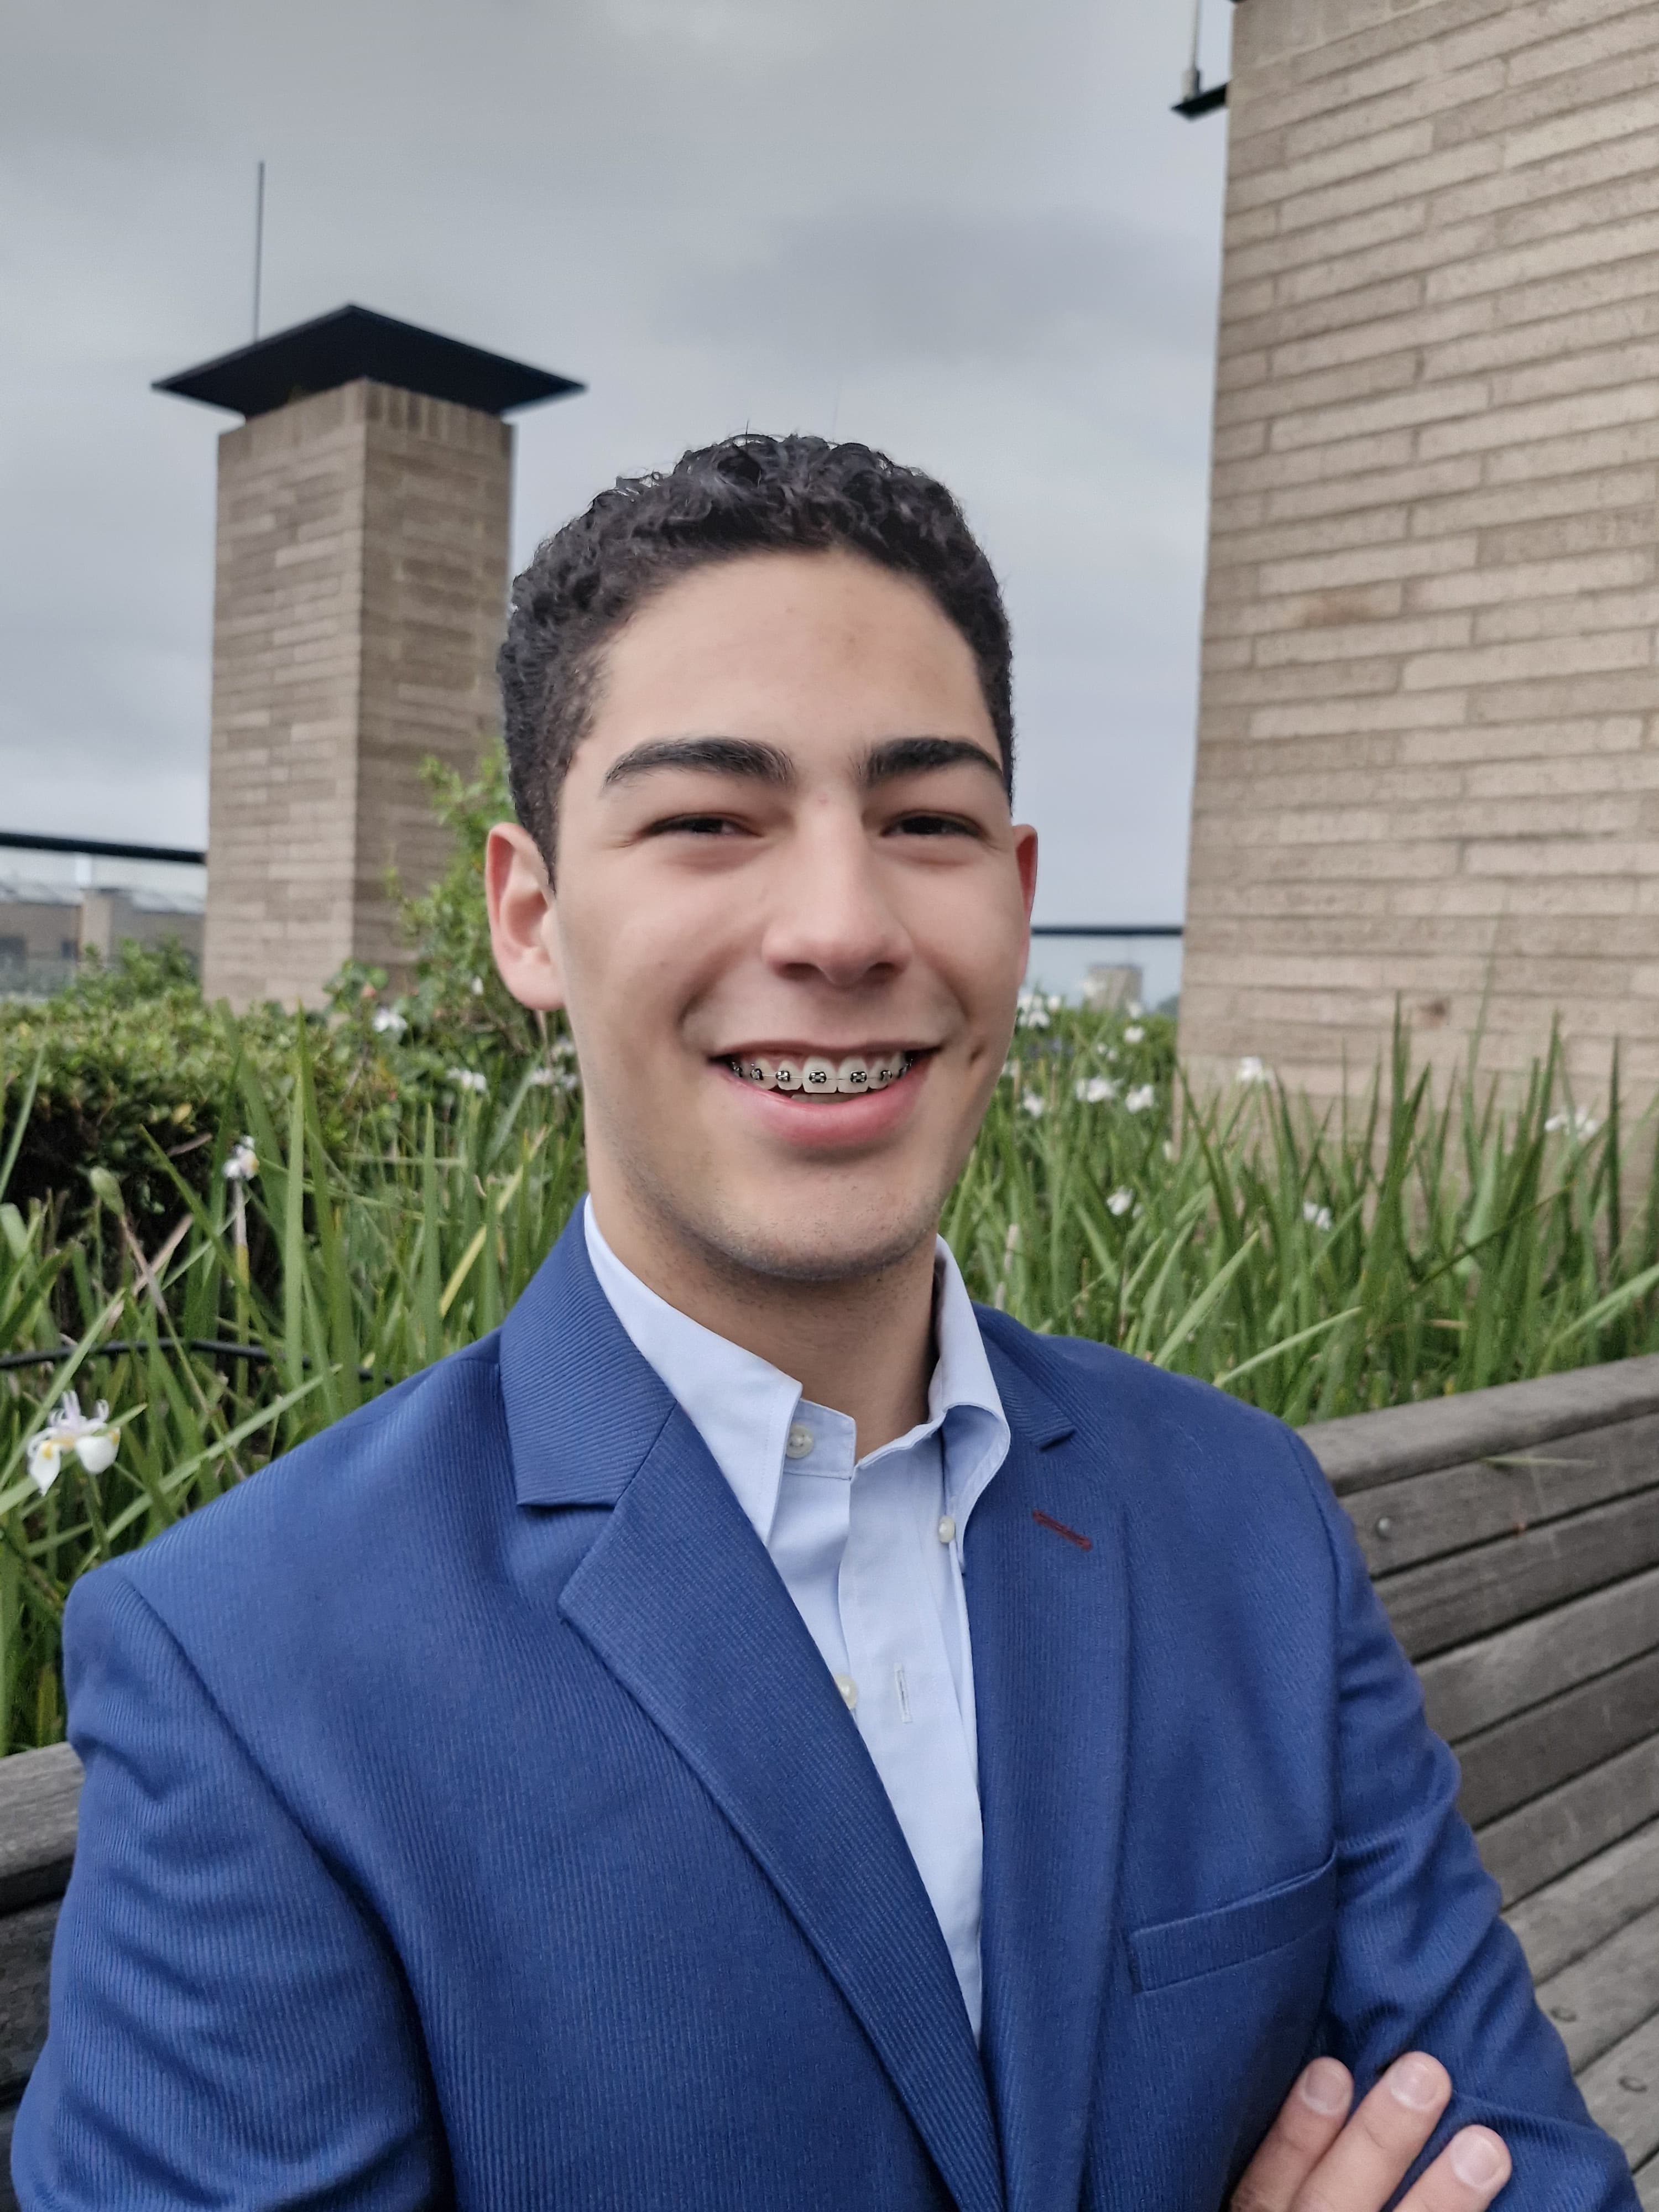
\includegraphics[scale=0.015]{Digital_photo.jpg}} & 
  \begin{tabular*}{\linewidth}{l@{\extracolsep{\fill}}r}
        
            \textbf{\Large \textcolor{mydarkgreen}{Javier Andrés TARAZONA JIMENEZ}} & \textbf{\textcolor{mydarkgreen}{Email:}} \href{mailto:jtarazonaj@unal.edu.co}{jtarazonaj@unal.edu.co}\\
            
            \footnotesize Systems and Computer Science Engineer - Artificial Intelligence & \href{mailto:javier-andres.tarazona@ensta-paris.fr}{javier-andres.tarazona@ensta-paris.fr}\\
            
            \href{https://www.linkedin.com/in/javier-andres-tarazona-jimenez-84b489222/}{\textcolor{blue}{\underline{LinkedIn}}} & \textbf{\textcolor{mydarkgreen}{Mobile:}} +33 07 46 36 97 75 \\

            \href{https://github.com/JavierTarazona06}{\textcolor{blue}{\underline{GitHub}}} & Palaiseau, Île de France, France (91120)\\
        \end{tabular*}
    \\
\end{tabularx}

\vspace{0.3cm}

\textbf{Seeking a 3-month research internship in Artificial Intelligence starting June 2026} 

%-----------EDUCATION-----------------
\section{\textcolor{mydarkgreen}{\textbf{Education}}}
  \resumeSubHeadingListStart
    \resumeSubheading
      {ENSTA Paris - Institut Polytechnique de Paris}{Paris, France}
  {\shortstack[l]{
    Diplôme d'Ingénieur - Specialization in AI - Master of Science in Engineering
    \\\underline{\textbf{Eiffel Excellence Scholarship \textendash{} Master's 2025\textendash{}2027}}}}{September 2025 -- Present}
    \resumeSubheading
      {Universidad Nacional de Colombia (UNAL)}{Bogotá, Colombia}
      {\shortstack[l]{Computer Science and Systems Engineering; GPA: 4.7/5.0
            \\\underline{\textbf{Tuition waiver for academic excellence} (2021\textendash{}2024)}}
        }{January 2021 -- July 2025}
    \resumeSubheading
      {University of Saskatchewan}{Saskatoon, Canada}
      {\shortstack[l]{\footnotesize Academic exchange.\\Advanced Software Engineering, 
       Algorithms, Operating Systems and French for Business}}{September 2024 -- December 2024}
    \resumeSubheading
      {Universidad de los Andes}{Bogotá, Colombia}
      {\footnotesize Academic exchange. Computer Networks}{January 2024 -- July 2024}
  \resumeSubHeadingListEnd


%-----------EXPERIENCE-----------------
\section{\textcolor{mydarkgreen}{\textbf{Experience}}}
  \resumeSubHeadingListStart
    \resumeSubheading
      {Engin A.I}{Bogotá, Colombia}
      {Software Engineer \& Computer Vision}{12 months: Jan - Jul 2024 and Feb - Jun 2025}
      \resumeItemListStart
        \resumeItem{Python development \& software design}
          {Refactored two libraries using object-oriented and modular design, optimizing image analysis and automating data processing 
          \textbf{(improved developer efficiency by 80 \% )}.}
        \resumeItem{Computer Vision (OpenCV, NumPy, mathematics)}
          {Improved a post-processing pipeline for lane and road marking detection, increasing speed by 
          \textbf{50\% and accuracy by 60\%}. Applied machine learning techniques (unsupervised clustering)
           to improve model robustness and performance.}
        \resumeItem{Data analysis and abstraction}
          {Generated wheel-path trajectories and correlated deterioration zones, improving overall system 
          performance and \textbf{user satisfaction (+10\%)}.}
      \resumeItemListEnd
  \resumeSubHeadingListEnd


%-----------PROJECTS-----------------
\section{\textcolor{mydarkgreen}{\textbf{Academic Projects}}}
  \resumeSubHeadingListStart

      \resumeSubheading
      {Slow}{}
      {Desktop application \textendash{} Python, MySQL, OpenCV}{}
      \resumeItemListStart
        \resumeItem{Video analysis and speed detection}
          {Designed and developed a system to analyze video and measure vehicle speed, improving traffic monitoring automation.}
      \resumeItemListEnd

      \resumeSubheading
      {ORIUN and Managy}{}
      {Python, Django, React, SQL, Docker, Google Cloud Platform (GCP)}{}
      \resumeItemListStart
        \resumeItem{Web and backend development}
          {Built two web management and booking platforms with a Django backend and cloud services (GCP).}
        \resumeItem{Architecture and project management}
          {Implemented a microservices architecture using Docker and coordinated development with agile (SCRUM).}
        \resumeItem{Real-time systems}
          {Integrated real-time booking features to improve user experience and reliability.}
        \resumeItem{Ideation, prototyping and communication}{
        ORIUN project supervised and validated by the Innovation Management Unit of the
        Universidad Nacional de Colombia.}
      \resumeItemListEnd

      \resumeSubheading
      {Sharp Sight}{}
      {FastAPI, Python, Web Scraping}{}
      \resumeItemListStart
        \resumeItem{API and data collection}
          {Developed a scalable API to compare prices of tech products via real-time scraping.}
      \resumeItemListEnd
      
  \resumeSubHeadingListEnd


%--------EXPERTISE------------
\section{\textcolor{mydarkgreen}{\textbf{Honors \& Skills}}}
{\begin{itemize}[leftmargin=*,itemsep=2pt,parsep=0pt,topsep=2pt,partopsep=0pt]
  \item{\textbf{Honorable Mention \textendash{} ICPC Colombia 2023} \newline XXXVII National Programming Marathon ACIS REDIS}
   \item{\textbf{AI Tools:} Python, Scikit-Learn, OpenCV, NumPy, Pandas.}
   \item{\textbf{AI \& Data Science:} Machine Learning, Data Analysis, Multi-Agent Systems.}
   \item{\textbf{Programming Software \& Cloud:} Cloud (GCP), Docker, Django, FastAPI, React, JavaScript, C++/C, Java, SQL/NoSQL.}
   \item{\textbf{Methodologies:} Agile (SCRUM), Git/GitHub, CI/CD, software architecture.}
   \item{\textbf{Languages:} English (C1 \textendash{} \textbf{IELTS 2024}), 
    French (B2 \textendash{} \textbf{DELF 2024}), Spanish (native).}
  \item{\textbf{Soft skills:} Leadership, resilience and cross-cultural communication (in international teams).}
\end{itemize}}


% (Interests moved to footer)

%-------------------------------------------
\end{document}
